% !TEX root = master.tex

\chapter{Model Order Reduction}
\label{Ch:ROM}
%\pagenumbering{arabic}

This chapter introduces model order reduction (MOR) of the BGK-model in the Sod's shock tube, for which POD and in particular autoencoders are adopted to obtain a reduced basis (RB).\\
Model order reduction is a technique used for reducing the computational cost when evaluating PDEs \cite{Bernard}\cite{Carlberg}\cite{ohlberger2015reduced}. To achieve this, the solution to a PDE is approximated by reducing one or more of its dimensions. The reduction performs a mapping onto a low-dimensional manifold. In this case the solution to the BGK model is a function \(f(x,v,t) \in \mathbb{R}^3\). For example,  \(v\) could be reduced to \(n\), where \(k\) represents the number of elements in \(v\) and \(p\) represents the number of elements in \(n\). With \(p << k\) we obtain a reduced order model (ROM) which we call \(q(x,n,t)\) of significantly lower dimension. In particular, \(n\) is called the reduced basis or the intrinsic variable. \Cref{Ch:BGK} shows that the BGK-model is a PDE which through discretization in the spatial dimension \(x\) and the velocity dimension \(v\) holds a system of \(KJ\) ODE's in time in 1D and \(K^3J^3\) ODE's in time in 3D.  By the reduction of \(v\), we arrive at \(nJ\) ODE' in time for 1D and \(nJ^3\) ODE's in time in 3D. This example illustrates the number of computations that can be saved by MOR. The mapping from \(f(x,v,t)\) to \(q(x,n,t)\) can be performed by one of the reduction algorithms from \cref{Ch:DimRedAl}. The remapping back to \(\tilde{f}(x,v,t)\) is carried out by the same algorithm under the condition, that the distance \(||f - \tilde{f}||\) is small.\\
\begin{figure}[H]
	\begin{subfigure}{.45\textwidth}
		\centering
		\tikzstyle{reco} = [rectangle,minimum height=4em,text centered, fill=blue!20,draw=black]
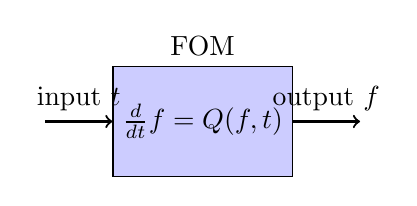
\begin{tikzpicture}[scale=0.5]
	\node [reco,label=FOM] (phys) {$\frac{d}{dt}f = Q(f,t)$};
	\draw [<-,thick] (phys)--+ (-4,0) node[midway,above] {input \(t\)};
	\draw [->,thick] (phys)--+ (4,0) node[midway,above] {output $f$};
\end{tikzpicture}

		\subcaption{Evolving the BGK model in Sod's shock tube in time is generated through evaluating the FOM in space \(x\), velocity \(v\) and time \(t\), which yields the solution \(f(x,v,t)\). The operator \(Q\) is here the FOM described in \cref{Ch:BGK}.}
	\end{subfigure}\hfill
	\begin{subfigure}{.45\textwidth}
		\centering
		\tikzstyle{reco} = [rectangle,minimum height=4em,text centered, fill=blue!20,draw=black]
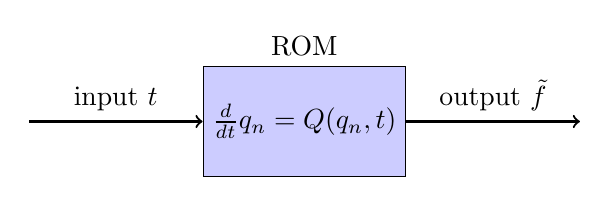
\begin{tikzpicture}[auto]
	\node [reco,label=ROM] (red) {$\frac{d}{dt}q_n = Q(q_n,t)$};
	\draw [<-,thick] (red)--+ (-3.5,0) node[midway,above] {input \(t\)};
	\draw [->,thick] (red)--+ (3.5,0) node[midway,above] {output $\tilde{f}$};
\end{tikzpicture}

		\subcaption{Evolving the ROM of the BGK model in Sod's shock tube in time through evaluating the ROM at \(n\) and \(\mu_i\) yields an approximation to the FOM solution \(\tilde{f}\). The operator \(Q\) is here either POD or an autoencoder described in \cref{Ch:DimRedAl}.}
	\end{subfigure}
	\caption{Outline of the correlation between the FOM solution and the approximation obtained from the ROM.}
\end{figure}
To summarize, the idea that every high dimensional dynamical-state space \(W\), also called solution
manifold, can be mapped onto a state-space i.e. V of lower dimension, is exploited within MOR \cite{ohlberger2015reduced}. Thus, \(f(x, v, t) \in W\) and \(q(n,\mu_i) \in V\), where \(\mu_i\) gives the variables omitted by the reduction and \(n\) the intrinsic variables. Again, p counts through the intrinsic variables. The state-space of the lower dimension is called the intrinsic solution manifold \(V\) with \(q(n, \mu_i) \in V\)\cite{Carlberg}.
MOR is partitioned into two successive phases called the \textit{offline} - and the \textit{online} phase. During the offline phase, experiments or simulations of the full order model (FOM) generate \textit{snapshots} of a dynamical system. The snapshots \(F = \{f(t_1),...,f(t_n)\}\) are created once, each representing one moment in time of the dynamical system. Thus a snapshot database of solutions \(f(x,v,t)\) of the BKG model in Sod's shock tube is required. Next the mapping \(Q\) is constructed such that \(\tilde{f} = Q(f)\), for which \(f(t_i) \approx \tilde{f}(t_i)\), reducing the dimensionality of the FOM solution as outlined before. During the online phase, the reduced-order model is evaluated and the error is estimated by
\begin{equation}
	\L2 = \frac{||f - \tilde{f} ||_2}{||f||_2}
\end{equation}
which is called the relative \(\L2\)-Error norm. Note, the abbreviation \(\L2\) is used from here on. Therefore the online phase may be described as a stage of independence from the full order model. Following \cite{ohlberger2015reduced} and \cite{Carlberg}, the success when building a ROM through linear reduction methods like the POD, depends on a rapidly decaying Kolmogorov N-width. In particular, advection-dominated problems exhibit a slow decay of the Kolmogorov N-width as described in \cite{ohlberger2015reduced}, thus yielding the need for non-linear methods like autoencoders. The Kolmogorov N-width is given by
\begin{equation}
	d_{V}(W):= \sup_{f \in W} \inf_{\tilde{f} \in V} ||f-\tilde{f}||
	\label{Eq:Kolmogorov}
\end{equation}
and measures the worst best-approximation error for elements of \(W\). The convergence behavior of the Kolmogorov N-width for advection-dominated problems, especially when jump conditions are involved as in Sod's shock tube, decays with
\begin{equation}
	d_p(W) \leq \frac{1}{2} p^{-1/2},
	\label{Eq:KolmoAdv}
\end{equation}
where \(p\) denotes the number of RB or intrinsic variables. Further insight is provided in \cite{ohlberger2015reduced}.\\
Note, that hereafter the term intrinsic variables will be used solely. The relevance of using non-linear reduction methods for MOR is often formulated in terms of a slow decaying Kolmogorov N-width. And even though the BGK-model in Sod's shock tube describes an advection problem with jump discontinuities implies that linear reduction methods should fail, the following will show that this is only partly true for this case.

\section{Offline phase and number of intrinsic variables}\label{Sec: FOM}

The FOM is the 1D BGK-model in Sod's shock tube for which solutions \(f(x,v,t)\) for two levels of rarefaction are gratefully provided by Julian K\"ollermeier and the Departement of Mathematics at the RWTH Aachen.\\
One level with \(\Kn=0.01\) can be viewed as a slip flow as explained in \cite{schaaf}. The dilution up to this level of rarefaction is little, though the boundary to view this flow as a continuum is reached, leading to inaccuracies when employing the common Navier Stokes equations. Still the NFS-equations (Navier-Stokes-Fourrier) could be used \cite{NumaKUL} in addition to the BGK-model. The solution with this level of rarefaction is hereafter referred to as \(\rare\). The other is a solution which is situated in the continuum flow regime with \(\Kn=0.00001\) for which the Navier-Stokes equations can be utilized without hesitation. Hereafter the solution for this flow will be referred to as \(\hy\). An in-depth description of the BGK-model and Sod's shock can be found in \cref{Ch:BGK}.\\
Note that both \(\hy\) and \(\rare\) are three dimensional tensors comprising \(f(x,v,t)\).\\
Sod's shock tube is discretized in space \(x\) with 100 nodes, in velocity \(v\) with 40 nodes for 25 time steps in time \(t\), as presented in \cref{Tab:Setup} and \cref{Fig:SodProbSetup}.
\begin{table}[htp]
	\centering
	\caption{Problem setup for the BGK model in Sod's shock tube. The diaphragm is positioned at \(x_d=0.5025\). For the initial condition with \(t=0\) the gas is present at \(x<x_d\) and absent for \(x\geq x_d\).}
	\begin{tabular*}{15cm}{ @{\extracolsep{\fill}} c c c c @{} }
		\toprule
		Variable   & Number of nodes \(i\)&   Domain extension& Step size (uniform)\\   
		\hline
		\(x\) 		&	200&     [0.0025,0.9975]&	    0.00499\\
		\(v\)       &   40 &  		    [-10,10]&	    \(\approx\) 0.51282051\\
		\(t\)   	&	25 &        	[0,0.12]&	      0.005\\
		\bottomrule
	\end{tabular*} \label{Tab:Setup}
\end{table}

The reduction algorithms, introduced in \cref{Ch:DimRedAl}, require a distinct reshaping of the input data before they can be used. The preprocessed matrix for the FCNN as one batch  \(\btchfc\), is shown in \cref{Eq:AE_matrix}. Each row of \(\btchfc\) represents \(\btchfc_{,l}=f(v,t_i,x_j)\), an example, that can be fed to the FCNN. Hence \(x_jt_i=5000\) samples can be acquired. POD can use \(\btchfc\) as well as \(P^T_{FCNN}\) it's transposition as input.\\
The preprocessed matrix for the CNN, \(\btchcn\), is shown in \cref{Eq:CNN_matrix} with \(\btchcn_{,l} = f(x,t,v_k)\). Hence \(v_k=40\) examples can be obtained to be fed into the CNN. Because of the little amount of available examples per rarefaction level, it is decided to combine \(\hy\) and \(\rare\) to one dataset, yielding 80 available examples for training the CNN. This measure leads to one model, that has the abillity to generalize about the BGK-model for a variety of rarefaction levels in Sod's shock tube. Details can be found in \cref{Ch:ApB}. In the following, a distinction between \(\btchcn\) and \(\btchfc\) is omitted, when referring to the preprocessed matrices\\
\begin{minipage}{.45\linewidth}
	\begin{gather}
	\btchfc = \begin{bmatrix}
	f(v_1,t_1,x_1)&\cdots &f(v_n,t_1,x_1) \\
	f(v_1,t_1,x_2)&\cdots &f(v_n,t_1,x_2) \\
	\vdots& \vdots & \vdots\\
	f(v_1,t_1,x_n)&\cdots &f(v_n,t_1,x_n)\\
	f(v_1,t_2,x_1)&\cdots &f(v_n,t_2,x_1)\\
	\vdots & \vdots & \vdots\\
	f(v_1,t_n,x_n)&\cdots &f(v_n,t_n,x_n)
	\end{bmatrix}
	%\raisetag{15pt}
	\label{Eq:AE_matrix}
	\end{gather}
\end{minipage},\qquad%
\begin{minipage}{.35\linewidth}
	\begin{gather}
	\btchcn= \begin{bmatrix}
	n_{Filters},&f(v_1,\textbf{t},\textbf{x})\\
	n_{Filters},&f(v_2,\textbf{t},\textbf{x})\\
	\vdots&\vdots\\
	n_{Filters},&f(v_n,\textbf{t},\textbf{x})
	\end{bmatrix}
	\label{Eq:CNN_matrix}
	\end{gather}
\end{minipage}\textrm{.}\\\\
With the FOM solution at hand it is possible to construct a mapping \(Q\) such that \(Q(f)\approx \tilde{f}\). Again,for \(Q\), POD and two autoencoders, the FCNN and the CNN, are employed. With considering \cref{Ch:ApA} and \cref{Ch:ApB}, the selection of hyperparameters and training for the FCNN and the CNN is discussed, providing fully trained and tuned FCNNs and a CNN, which are considered as given from now on.\\
Note that since this thesis focuses on the use of neural networks, POD acts as a benchmark. Consequently, in oder to contrast the number \(p\) of intrinsic variables of the autoencoders (sizes of the code layer) we will utilize POD as a reference framework. The intrinsic variables obtained from POD, the FCNN and the CNN, will be referred as \(\idhy\) and \(\idrare\), where the former describes the intrinsic variables when reducing \(\hy\) and the latter when reducing \(\rare\).\\
A first step is to perform a POD with \(\hy\) and \(\rare\) distinctively. The obtained singular values \(\sigma\), as well as the cumulative energy (cusum-e), which is defined as\\
\noindent \begin{minipage}{.3\linewidth}
	\begin{equation}
	\textrm{cusum-e} = \frac{\textrm{cusum}}{\sum_i \sigma_i}
	\end{equation}
\end{minipage}%
\begin{minipage}{.7\linewidth}
	\begin{equation}
			\textrm{with} \qquad\qquad(\textrm{cusum})_i =(\text{cusum})_{i-1} + \sigma_{i}
	\end{equation}
\end{minipage},\\\\
over the singular values, are shown in \cref{Fig:CUSUM-e}. With a total of \(p=4\) intrinsic variables, a cumulative energy of over \(99\%\) can be achieved for \(\hy\). The fourth singular value measures to a value of \(\sigma_4 = 0.706\). The cumulative energy of the singular values of \(\rare\) arrives above \(99\%\) with \(p=6\) singular values. The sixth value is at \(\sigma_6 = 0.275\). Thus a slight difference can be observed for both datasets when emplying POD.\\
We can link the decay of the Kolmogorov N-width in \cref{Eq:Kolmogorov} with the decay of the singular values, which invalidates the application of \cref{Eq:KolmoAdv} for the FOM solutions.  The rate at which the singular values drop is approximately exponential in \(\hy\) and in \(\rare\) and in turn indicates a rapid decay of the Kolmogorov N-width. Hence supports the  assumption that advection and sharp shock fronts do not appear predominantly. The eventough small, but dissimilar, decay rate of the singular values is a manifestation of the different rarefaction levels: With a decreasing number of particles present in Sod's shock tube, the lesser the probability of a single bulk macroscopic behavior emerges as seen in the full survey of the BGK model in \cref{Ch:BGK}, leading to an expected increased number of intrinsic variables necessary to achieve similar \(\L2\)-errors.  
\begin{figure}[H]
	\begin{subfigure}{.45\textwidth}
		% This file was created by tikzplotlib v0.9.6.
\begin{tikzpicture}

\begin{groupplot}[group style={group size=2 by 1, horizontal sep=1cm, vertical sep=2cm}]
\nextgroupplot[
log basis y={10},
tick align=outside,
tick pos=left,
x grid style={white!69.0196078431373!black},
xlabel={\(k\)},
xmin=-0.95, xmax=41.95,,
xtick style={color=black},
y grid style={white!69.0196078431373!black},
ylabel={\(\sigma\)},
ymin=2.86160392849359e-16, ymax=240.32740800328,
ymode=log,
ytick style={color=black},
ytick={1e1,1e-3,1e-11,1e-15},
width=.55\textwidth,
height=.7\textwidth,
y label style={yshift=-2.5em},
grid=both
]
\addplot [semithick, red, mark=o, mark size=2, mark options={solid}]
table {%
1 36.8185958349281
2 5.78483852846218
3 2.9488881352441
4 1.08115123432794
5 0.4715894924307
6 0.27551553286601
7 0.155493855631619
8 0.0601331453526982
9 0.05155511017701
10 0.0132542951500055
11 0.0118122790965581
12 0.00208495452053553
13 0.00184461993287337
14 0.000261109297076443
15 0.000174118703867616
16 2.59262125849959e-05
17 1.30752219185821e-05
18 1.92140998809572e-06
19 9.1685066176197e-07
20 1.08651788755093e-07
21 5.26354986735524e-08
22 4.52124036969183e-09
23 2.44729256168519e-09
24 1.43747068296607e-10
25 9.28350136149776e-11
26 3.39879764456285e-12
27 2.74182349854538e-12
28 6.4789443879917e-14
29 6.12293316992491e-14
30 1.6313694307166e-14
31 2.92181471455653e-15
32 2.92181471455653e-15
33 2.92181471455653e-15
34 2.92181471455653e-15
35 2.92181471455653e-15
36 2.92181471455653e-15
37 2.92181471455653e-15
38 2.92181471455653e-15
39 2.92181471455653e-15
40 1.8678655154319e-15
};

\nextgroupplot[
tick align=outside,
tick pos=left,
x grid style={white!69.0196078431373!black},
xlabel={\(k\)},
xmin=-0.95, xmax=41.95,
xtick style={color=black},
y grid style={white!69.0196078431373!black},
ylabel={cusum-e},
ymin=0.760859233580134, ymax=1.0113876555438,
ytick style={color=black},
ytick={1,.8},
width=.55\textwidth,
height=.7\textwidth,
y label style={yshift=-2em},
grid=both
]
\addplot [semithick, red, mark=o, mark size=2, mark options={solid}]
table {%
1 0.772246889123937
2 0.893580238655189
3 0.95543131247198
4 0.978107779579132
5 0.987999072557982
6 0.993777837563443
7 0.997039223381299
8 0.998300478281949
9 0.999381814290284
10 0.999659814794242
11 0.999907569918492
12 0.999951300528145
13 0.99998999027099
14 0.999995466874262
15 0.999999118904556
16 0.999999662690558
17 0.999999936935114
18 0.99999997723548
19 0.999999996465846
20 0.999999998744749
21 0.999999999848745
22 0.999999999943575
23 0.999999999994906
24 0.999999999997921
25 0.999999999999868
26 0.999999999999939
27 0.999999999999997
28 0.999999999999998
29 0.999999999999999
30 1
31 1
32 1
33 1
34 1
35 1
36 1
37 1
38 1
39 1
40 1
};
\addplot [thick, , mark=x,black, mark size=2, mark options={solid}]
table{%
6 0
6 0.993777837563443
6 1.3
};
\end{groupplot}
\end{tikzpicture}


		\subcaption{Sigular values \(\sigma\) over \(k\) number of singular values (left) and cumulative energy, here labeled as \glqq cusum-e\grqq{} over \(k\) (right) for \(\hy\). A black cross marker corresponds to over 99\% cumulative energy.}
		\label{Fig:CumSum_Rare}
	\end{subfigure}\hfill
	\begin{subfigure}{.45\textwidth}
		% This file was created by tikzplotlib v0.9.6.
\begin{tikzpicture}

\begin{groupplot}[group style={group size=2 by 1, horizontal sep=1cm, vertical sep=2cm}]
\nextgroupplot[
log basis y={10},
tick align=outside,
tick pos=left,
x grid style={white!69.0196078431373!black},
xlabel={\(k\)},
xmin=-0.95, xmax=41.95,,
xtick style={color=black},
y grid style={white!69.0196078431373!black},
ylabel={\(\sigma\)},
ymin=2.86160392849359e-16, ymax=240.32740800328,
ymode=log,
ytick style={color=black},
ytick={1e1,1e-3,1e-11,1e-15},
width=.55\textwidth,
height=.7\textwidth,
y label style={yshift=-2.5em},
grid=both
]
\addplot [semithick, red, mark=o, mark size=2, mark options={solid}]
table {%
1 36.8185958349281
2 5.78483852846218
3 2.9488881352441
4 1.08115123432794
5 0.4715894924307
6 0.27551553286601
7 0.155493855631619
8 0.0601331453526982
9 0.05155511017701
10 0.0132542951500055
11 0.0118122790965581
12 0.00208495452053553
13 0.00184461993287337
14 0.000261109297076443
15 0.000174118703867616
16 2.59262125849959e-05
17 1.30752219185821e-05
18 1.92140998809572e-06
19 9.1685066176197e-07
20 1.08651788755093e-07
21 5.26354986735524e-08
22 4.52124036969183e-09
23 2.44729256168519e-09
24 1.43747068296607e-10
25 9.28350136149776e-11
26 3.39879764456285e-12
27 2.74182349854538e-12
28 6.4789443879917e-14
29 6.12293316992491e-14
30 1.6313694307166e-14
31 2.92181471455653e-15
32 2.92181471455653e-15
33 2.92181471455653e-15
34 2.92181471455653e-15
35 2.92181471455653e-15
36 2.92181471455653e-15
37 2.92181471455653e-15
38 2.92181471455653e-15
39 2.92181471455653e-15
40 1.8678655154319e-15
};

\nextgroupplot[
tick align=outside,
tick pos=left,
x grid style={white!69.0196078431373!black},
xlabel={\(k\)},
xmin=-0.95, xmax=41.95,
xtick style={color=black},
y grid style={white!69.0196078431373!black},
ylabel={cusum-e},
ymin=0.760859233580134, ymax=1.0113876555438,
ytick style={color=black},
ytick={1,.8},
width=.55\textwidth,
height=.7\textwidth,
y label style={yshift=-2em},
grid=both
]
\addplot [semithick, red, mark=o, mark size=2, mark options={solid}]
table {%
1 0.772246889123937
2 0.893580238655189
3 0.95543131247198
4 0.978107779579132
5 0.987999072557982
6 0.993777837563443
7 0.997039223381299
8 0.998300478281949
9 0.999381814290284
10 0.999659814794242
11 0.999907569918492
12 0.999951300528145
13 0.99998999027099
14 0.999995466874262
15 0.999999118904556
16 0.999999662690558
17 0.999999936935114
18 0.99999997723548
19 0.999999996465846
20 0.999999998744749
21 0.999999999848745
22 0.999999999943575
23 0.999999999994906
24 0.999999999997921
25 0.999999999999868
26 0.999999999999939
27 0.999999999999997
28 0.999999999999998
29 0.999999999999999
30 1
31 1
32 1
33 1
34 1
35 1
36 1
37 1
38 1
39 1
40 1
};
\addplot [thick, , mark=x,black, mark size=2, mark options={solid}]
table{%
6 0
6 0.993777837563443
6 1.3
};
\end{groupplot}
\end{tikzpicture}


		\subcaption{Sigular values \(\sigma\) over \(k\) number of singular values (left) and cumulative energy, here labeled as \glqq cusum-e\grqq{} over \(k\) (right) for \(\rare\).  A black cross marker corresponds to over 99\% cumulative energy.}
		\label{Fig:CumSum_Hydro}
	\end{subfigure}
	\caption{Comparison of singular variables \(\sigma\) and cumulative energy for \(\hy\) and \(\rare\). The decay of the singular values can be used to estimate the decay of the Kolmogorov n-width.}
	\label{Fig:CUSUM-e}
\end{figure}
From a fluid mechanical point of view, the number of intrinsic variables for \(\hy\) in theory suffices with \(p=3\), as a slip-flow can be described in terms of three macroscopic quantities i.e. density \(\rho\), macroscopic velocity \(u\) and total energy \(E_{tot}\)as described in \cref{Eq:Conservation1} to \cref{Eq:Conservation3} and in \cite{BGK}\cite{Bernard}. As mentioned before, does theoretically \(\rare\) require \(p\) to be of a larger number as more than a single maxwellian describe the microscopic velocities. Therefore \(\idhy\) with \(p=3\) is employed and the FCNN is arranged in that way as a a starting value for the hyperparameter search. A starting value of \(p=5\) on the other hand is chosen for \(\idrare\). Note that this implies, that the CNN, which is trained with both rarefaction levels simultaneously, initially uses \(p=5\). The same value for \(p\) is chosen for the FCNN and \(\rare\).\\
In oder to shed light into the performance of the autoencoders with a different number sizes for \(\idhy\) and \(\idrare\), the size of the bottleneck layer of the autoencoders, which is the same as \(p\), are varied in a next step.\\
To this end $p$ is varied for POD, FCNN and CNN over $p \in \{1,2,4,8,16,32\}$ for both rarefaction levels. Note that the neural networks needed to be trained for these experiments and that by changing $p$ i.e. widening the bottleneck layer, a gain or loss of capacity occurs which can be connected to stability during training, see \cref{Ch:DimRedAl} and \cite{Goodfellow}.
\begin{figure}[htbp!]
	% This file was created by tikzplotlib v0.9.6.
\begin{tikzpicture}
\definecolor{color0}{rgb}{0.12156862745098,0.466666666666667,0.705882352941177}

\begin{groupplot}[group style={group size=2 by 1,horizontal sep=2cm}]
\nextgroupplot[
legend cell align={left},
legend style={draw=none,at={(0.03,0.03)}, anchor=south west},
log basis y={10},
tick align=outside,
tick pos=left,
x grid style={white!69.0196078431373!black},
xmajorgrids,
xmin=-0.55, xmax=33.55,
xminorgrids,
xtick style={color=black},
y grid style={white!69.0196078431373!black},
ymajorgrids,
ymin=4.38349387313967e-16, ymax=1.61134858880557,
yminorgrids,
ymode=log,
ytick style={color=black},
ytick={1e-1,1e-2,1e-3,1e-4,1e-6,1e-8,1e-10,1e-12,1e-14},
xlabel={Number of intrinsic varibales},
ylabel={\(L_2\)-Error},
width=0.47\textwidth,
height =.45\textwidth,
clip=false,
y label style={yshift=-.7em},
max space between ticks=20
]
\addplot [thick, red, mark=o, mark size=2, mark options={solid}, dashed]
table {%
1 0.188112310801957
2 0.0750338979596223
3 0.020528730333796635
4 0.00808627149114823
8 0.000193252431896578
16 3.06183124046159e-08
32 2.23530701528268e-15
};
\addlegendentry{POD}
\addplot [thick, color0, mark=pentagon, mark size=2, mark options={solid}, only marks]
table {%
1 0.00663323979824781
2 0.00234045716933906
3 0.0008
4 0.000691965571604669
8 0.000261269917245954
16 0.000194361884496175
32 0.000206562195671722
};
\addlegendentry{FCNN}
\addplot [thick, green!50!black, mark=triangle, mark size=2, mark options={solid,rotate=180}, only marks]
table {%
1 0.176033899188042
2 0.0960375890135765
4 0.0284016542136669
5 0.026
8 0.0258560031652451
16 0.0232554506510496
32 0.0237289071083069
};
\addlegendentry{CNN}
\draw[thick](3,40e-17)--(3,1.5);
\draw [thick,<-] (axis cs:3,1.5)-- +(10pt,10pt) node[right] {\(p\)};
\nextgroupplot[
legend cell align={left},
legend style={draw=none, at={(0.03,0.03)}, anchor=south west},
log basis y={10},
tick align=outside,
tick pos=left,
x grid style={white!69.0196078431373!black},
xmajorgrids,
xmin=-0.55, xmax=33.55,
xminorgrids,
xtick style={color=black},
y grid style={white!69.0196078431373!black},
ymajorgrids,
ymin=1.70008814466799e-15, ymax=0.821373329691319,
yminorgrids,
ymode=log,
ytick style={color=black},
ytick={1e0,1e-1,1e-2,1e-3,1e-4,1e-6,1e-8,1e-10,1e-12,1e-14},
xlabel={Number of intrinsic varibales},
ylabel={\(L_2\)-Error},
width=0.47\textwidth,
height =.45\textwidth,
clip=false,
y label style={yshift=-.7em},
max space between ticks=20
]
\addplot [thick, red, mark=o, mark size=2, mark options={solid}, dashed]
table {%
1 0.176637499442346
2 0.0853532495802733
4 0.015335605212791
5 0.008731715326052242
8 0.00145958547754045
16 3.54159334428613e-07
32 7.90549608414532e-15
};
\addlegendentry{POD}
\addplot [thick, color0, mark=pentagon, mark size=2, mark options={solid}, only marks]
table {%
1 0.58092600107193
2 0.00492882402613759
4 0.0029036
5 0.0009
8 0.00120856
16 0.000355097494320944
32 0.000395381561247632
};
\addlegendentry{FCNN}
\addplot [thick, green!50!black, mark=triangle, mark size=2, mark options={solid,rotate=180}, only marks]
table {%
1 0.160851925611496
2 0.0912962183356285
4 0.0309077128767967
5 0.026
8 0.0263328477740288
16 0.0228330623358488
32 0.022412983700633
};
\addlegendentry{CNN}
\draw[thick](5,16.5e-16)--(5,0.85);
\draw [thick,<-] (axis cs:5,0.85)-- +(10pt,10pt) node[right] {\(p\)};
\end{groupplot}

\end{tikzpicture}

	\caption{Variation of the number of intrinsic variables \(p\) over the $\L2$-Error for POD, FCNN and CNN. Results for $\hy$ are displayed on the left and for $\rare$ on the right.}
	\label{Fig:IntVar}
\end{figure}
Shown in \cref{Fig:IntVar} is the outcome of said experiments. The design for \cref{Fig:IntVar} is taken from \cite{Carlberg}. The loss of information when applying POD goes exponentially to zero with increasing $p$ which is not suprising when consulting the \textit{Eckard-Young Theorem} provided in \cref{Eq:EckardYoung} taken from \cite{Kutz}.
The left plot of \cref{Fig:IntVar} displays the results for $\hy$ with $p=3$ the estimated size of \(\idhy\), emphasized with a black line. The \(\L2\)-error of the FCNN first drops until $p = 3$ reaching \(\L2 = 0.0008\) to then drop further until \(p=8\) with \(\L2=0.00026\). Afterwards the \(\L2\) stagnates with a best value of \(\L2=0.00019\) at \(p=16\). Interestingly, the biggest improvement can be observed until \(p=3\).\\
The \(\L2\)-error of the CNN, that was trained with both rarefaction levels, drops until \(p=4\) reaching \(\L2=0.028\). Afterwards the \(\L2\)-error stagnates reaching it's best value of \(\L2=0.023\) at \(p=16\) and \(p=32\). One can assume, that the value of the \(\L2\)-error is approximately the same for \(p=3\) and \(p=4\), as it is for the FCNN. Therefore the CNN, as well as the FCNN, seem to reflect the assumptions for \(p\) considering \(\hy\). While the CNN and POD are congruent for \(p=1\) and \(p=2\) with POD outperfoming the CNN afterwards, the FCNN is only outperformed by POD after \(p=8\), where the \(\L2\)-error of both algorithms meet.\\ 
Moving forward, to assess the value of \(p\) for $\rare$ consider the right plot of \cref{Fig:IntVar}. Again \(p=5\) is highlited with a black line to indicate it's assumed value. The $\L2$-Error of the FCNN begins as the highest of all three algorithms with \(\L2=0.58\) at \(p=1\). Afterwards the \(\L2\)-error plummets outperforming POD and the CNN until \(p=8\). After \(p=8\), where POD and the FCNN meet with \(\L2=0.012\) and \(\L2=0.014\) respectively, POD outperforms both algorithms. From \(p=4\) to \(p=5\) the \(\L2\)-error of the FCNN drops from \(\L2=0.0029\) to \(\L2=0.0009\). The increase in \(\L2\)-error moving from $p=5$ to $p=8$ is not an result of overfitting as seen in \cref{Ch:ApB}, and therefore can only be explained with a bad initialization point of the networks free parameters $\frepar$. A continued widening of the bottleneck layer results in the lowest error of \(\L2=0.00035\) at \(p=16\) for the FCNN.\\
Resulting \(\L2\)-error values of POD and the CNN match for \(p=1\) and \(p=2\). Thereafter the error drops to \(\L2=0.03\) and \(\L2=0.026\) for \(p=4\) and \(p=5\) respectively. Continuing to widen the bottleneck layer one can observe, that the \(\L2\)-error stagnates. Nevertheless, the lowest error is reached with \(\L2=0.022\) at \(p=16\) and \(p=32\).\\
The variation of \(p\) shows that for the assumed values of \(p=3\) and \(p=5\) the FCNN outperforms POD. Additionally, the performance of both autoencoders increases up to those points, which accentuates the previously made assumptions for \(p\). Nonetheless, those are not the lowest values the FCNN, and with some limitations also the CNN, can reach. Until \(p=8\) the FCNN reaches it's limitations for surpassing POD. Hence, depending on \(p\) either POD or the FCNN have the ability to surpass each other. In order to evaluate the interpretability of all three algorithms, \(p=3\) and \(p=5\) is chosen for sizes of \(\idhy\) and \(\idrare\) respectively.\\

The following chapter covers the discussion of results obtained from POD, the FCNN and the FCNN. Additionally the evaluation of new states of the FOM is offered, which can be viewed as the online phase of MOR. 
 